\section{The Generator}
\label{sec:generator}

\generator{} is a forward-sampling generative model: a directed acyclic graph
(DAG) of samplers and renderers executed in topological order, in which every
random draw is taken from a named, seed-derived substream. This section
describes the layers in execution order; Figure~\ref{fig:pipeline} gives the
overview.

\begin{figure*}[t]
  \centering
  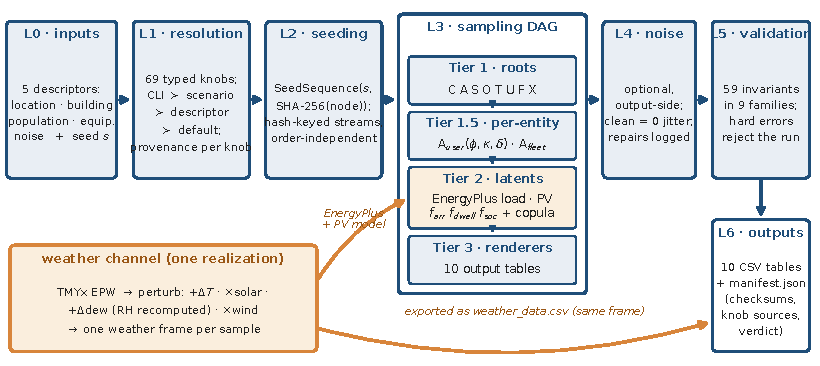
\includegraphics[width=\textwidth]{figures/fig1_pipeline.pdf}
  \caption{Pipeline overview. Five scenario descriptors and one seed resolve
  into a typed configuration; a sampling DAG produces latent variables and
  renders ten output tables; optional output-side noise, feasibility checks,
  and validation follow; a provenance manifest seals the run. A single
  perturbed weather realization (left) drives the building simulation, the PV
  model, and the exported weather channel.}
  \label{fig:pipeline}
\end{figure*}

\subsection{Scenario configuration and provenance}
\label{sec:knobs}

A scenario names five \emph{descriptors}---location, building, population,
equipment, and noise---each an entry in a small library, plus an optional set
of overrides. Descriptors expand into a flat namespace of 69 typed
configuration parameters (``knobs''), each with a declared type, range, and
default. Resolution follows a strict priority: command-line override
$\succ$ scenario override $\succ$ descriptor expansion $\succ$ registry
default. Every resolved value is stored with its source label (explicit,
descriptor, calibration provenance, or default), so the manifest of any
generated dataset answers, for all 69 parameters, \emph{why} each value is
what it is. Calibrated behavioral parameters
(\S\ref{sec:calibration}) enter through the same mechanism as
range-validated leaves carrying their calibration provenance; an out-of-range
override is rejected rather than clamped.

\subsection{Deterministic, order-independent randomness}
\label{sec:seeding}

All randomness derives from one integer seed $s$. Each DAG node $v$ draws from
a generator initialized with
$\mathrm{SeedSequence}(s,\ \mathrm{key}=h(v))$, where $h$ is a 32-bit digest
of the node \emph{name} (SHA-256 truncation); per-vehicle streams append the
vehicle index, and the session sampler keys additionally on the calendar day.
Because keys are content hashes rather than spawn order, adding a node to the
graph cannot shift any existing node's stream: datasets are bitwise
reproducible across generator versions that do not deliberately change a
sampler. Regression tests assert byte-identical output for fixed
$(\text{scenario}, s)$.

\subsection{Building load: simulated physics under controlled weather}
\label{sec:building}

The building channel is produced by EnergyPlus. The archetype and size
descriptors select an ASHRAE 90.1-2019 DOE prototype model (small, medium, or
large office; strip-mall or standalone retail; a mixed archetype averages an
office and a retail run). The location descriptor selects a
typical-meteorological-year (TMYx) weather file. Before simulation, the
weather is perturbed by four controlled channels: an additive dry-bulb offset
$\Delta T$, a multiplicative solar scale on the irradiance components, an
additive dew-point offset with relative humidity recomputed for thermodynamic
consistency (Magnus formula), and a multiplicative wind-speed scale. The
simulation runs at a fifteen-minute timestep and reports eight end-use meters,
which we aggregate into a \emph{flexible} component (cooling, heating, fans,
water systems---loads a building controller could in principle shift) and an
\emph{inflexible} component (interior and exterior lighting and plug loads).
Meter energies $E_J$ (joules per 900\,s interval) convert to mean interval
power as $P = E_J / (900 \times 1000)$~kW. A configuration switch either
normalizes the profile so that its peak equals the descriptor's design peak
(useful for controlled cross-scenario comparisons) or passes raw simulated
magnitudes through (used for all fidelity evaluation in
\S\ref{sec:representativeness}).

Two properties of this layer matter downstream. First, the \emph{same}
perturbed weather frame is consumed by the building simulation and the PV
model and is exported as the dataset's weather channel, so the released
channels are mutually consistent by construction. Second, weather perturbation
is \emph{input-side} variance: in multi-sample generation each sample draws
its own perturbation and is re-simulated, yielding physically faithful
sample-to-sample variability that cannot violate any downstream constraint.

\subsection{Drivers, vehicles, and charging sessions}
\label{sec:sessions}

\paragraph{Behavioral coordinates.}
Each driver is described by three axes: plug-in frequency
$\phifreq \in [0,1]$ (probability of appearing on a workday), timing
consistency $\kapcons \in [0,1]$, and daily distance $\deldist$ (km). A
\emph{population} is a weighted set of axis-aligned regions (boxes) in this
space. A driver is assigned a region categorically by weight, draws
$(\phifreq, \kapcons, \deldist)$ uniformly within the region's bounds, a
negotiation type from an empirical four-cluster mix, and a vehicle battery
class (24--100\,kWh) from the fleet mix.

\paragraph{Per-region distributions.}
Each region carries distribution parameters for arrival hour (truncated
normal, or a $k$-component truncated-normal mixture), dwell duration (Weibull,
or a two-component Weibull mixture), and the two SoC quantities (Beta
distributions), together with a Gaussian-copula correlation $\rho$ linking
arrival and dwell. When a population is calibrated
(\S\ref{sec:calibration}) these parameters are fitted values with recorded
provenance; hand-specified populations carry domain-informed values labeled
as such.

\paragraph{Session synthesis.}
For each vehicle and each eligible day, the vehicle appears with probability
$\phifreq$ (weekends scaled by a calibrated factor). On appearance, one joint
draw is made: a copula pair $(u_a, u_d)$ with correlation $\rho$ is
transformed through the inverse cumulative distribution functions of the
arrival and dwell marginals (mixtures are inverted by bisection on the
monotone mixture CDF, preserving the one-uniform-per-draw discipline that
determinism requires); arrival SoC and the required departure SoC are drawn
from their Beta marginals. The candidate session must then pass six
feasibility gates, evaluated atomically:
\begin{enumerate}
\item \emph{same-day}: departure falls on the arrival's calendar day;
\item \emph{window}: the session lies within the simulated horizon;
\item \emph{non-overlap}: arrival does not precede the vehicle's previous
  departure;
\item \emph{SoC monotonicity} (D6): required departure SoC strictly exceeds
  arrival SoC;
\item \emph{behavioral floor} (D7): required departure SoC meets the
  population's minimum-departure prior (active for hand-specified
  populations; calibrated cohorts set the floor to zero so fitted
  distributions are not clamped);
\item \emph{energy reachability} (D5):
  $\frac{(r - a)}{100}\,C \;\le\; P_{\max}\, \tau$,
  where $r$ and $a$ are required and arrival SoC (\%), $C$ the battery
  capacity (kWh), $P_{\max}$ the maximum charger rate (kW), and $\tau$ the
  dwell (h).
\end{enumerate}
A failed gate rejects the entire draw; after five rejections the vehicle-day
is dropped. Feasibility is thus enforced by \emph{rejection, never by
clamping}, so the emitted marginals are the fitted families conditioned on
feasibility rather than distorted by projection.

\subsection{Tariffs, demand response, PV, and storage}
\label{sec:der}

The tariff channel renders the location descriptor's rate structure (flat or
time-of-use with a peak window; a demand charge is carried as metadata for
downstream cost models). DR events are sampled from an inhomogeneous Poisson
process by thinning \citep{lewis1979thinning}: a base rate is modulated by
program season, weekday preference, a daily-maximum-temperature ramp driven
by the same weather realization, and a time-of-day window, then capped by
per-program monthly and seasonal limits; each program (CBP, BIP, ELRP)
carries its notification lead time. PV generation follows the PVWatts v5
chain \citep{dobos2014pvwatts}: plane-of-array irradiance by isotropic
transposition from the perturbed weather, cell temperature by the NOCT model,
temperature-derated DC power, and inverter-clipped AC power; the model is
deterministic, so PV varies across samples only through weather. Stationary
storage is released as a specification (capacity, power, efficiency, SoC
window)---deliberately without a dispatch schedule, since dispatch is a
decision of the downstream controller under evaluation, not exogenous data;
the same reasoning leaves charging \emph{schedules} out of the vehicle
tables.

\subsection{Output-side noise (optional)}
\label{sec:noise}

Separate from input-side weather variance, an optional noise layer perturbs
the \emph{rendered} tables to emulate measurement error: multiplicative
Gaussian jitter on load and prices, arrival-time jitter, arrival-SoC jitter,
and DR-notification dropout, in named profiles from ``clean'' (all zero; the
default, and the setting for every evaluation in this paper) to
``adversarial.'' Jitter can push a session past the sampler's feasibility
gates, so the layer re-clamps orderings and repairs reachability, recording
every repair in the manifest. Because repairs alter the guaranteed-feasible
contract, multi-sample corpora are generated with the clean profile and
input-side weather variance instead.

\subsection{Validation and the manifest}
\label{sec:validation}

Before a run is accepted, the generator checks the rendered tables against a
catalog of 59 invariants in nine families: schema, referential integrity,
temporal consistency (including same-day and non-overlap), SoC physics
(including reachability), charger conventions, behavioral-axis bounds,
CONSENT-share consistency, tariff and DR rules, and manifest integrity
(row counts and SHA-256 checksums). Charger-concurrency feasibility is
additionally measured and reported. The manifest records the full resolved
configuration with sources, generator version and git revision, per-file
checksums, feasibility metrics, any noise repairs, and the validation verdict
--- making every released file auditable and every run regenerable.
